\textbf{B.5.1--2. Input data and properties.} I use $L=14.0\ \mathrm{mm}$, $h=0.300\ \mathrm{mm}$, $b=0.750\ \mathrm{mm}$, $E=200\ \mathrm{GPa}$, $\rho=7850\ \mathrm{kg/m^3}$, $w_{\max}=0.150\ \mathrm{mm}$, and $N=5$. With bending about the axis associated with thickness $h$,
\[
A=bh=0.225\ \mathrm{mm^2},\quad m=\rho A=1.766\ \mathrm{g/m},\quad
I=\frac{bh^3}{12}=1.6875\times10^{-15}\ \mathrm{m^4}.
\]
\[
EI=0.3375\ \mathrm{mN\,m^2},\qquad a=(EI/m)^{1/4}=0.661\ \mathrm{m/\sqrt{s}}.
\]

\textbf{B.5.3--4. Eigenvalues and frequency.} The cantilever condition is $1+\cos z\cosh z=0$. Solving its equivalent bounded form $\cos z+\operatorname{sech}z=0$ gives the roots below. The frequency follows from $\omega_j=a^2(z_j/L)^2$.
\[
\begin{array}{c|rrrrr}
j&1&2&3&4&5\\\hline
z_j&1.8751&4.6941&7.8548&10.9955&14.1372\\
f_j\,(\mathrm{Hz})&1248&7821&21899.8&42914.9&70941.4
\end{array}
\]
Thus $f_1=1.248\ \mathrm{kHz}$, the nearest equal-tempered note is D\ensuremath{\sharp}6, and $\tau_1=0.8013\ \mathrm{ms}$.

\textbf{B.5.5--8. Modal expansion.} The course notes give the cantilever shape and plucked-reed initial condition (PDF pp. 184, 214--216). With $s=x/L$ and $\beta_j=(\cosh z_j+\cos z_j)/(\sinh z_j+\sin z_j)$,
\[
W_j(s)=\cosh(z_js)-\cos(z_js)-\beta_j[\sinh(z_js)-\sin(z_js)],
\quad w_0(s)=w_{\max}\left(\frac32s^2-\frac12s^3\right).
\]
The initial velocity is zero. I calculate the coefficients by numerical integration and then evaluate the tip displacement through three fundamental periods.
\[
A_j=\frac{\int_0^L w_0(x)W_j(x)\,dx}{\int_0^L W_j^2(x)\,dx},
\qquad w(L,t)=\sum_{j=1}^5 A_jW_j(L)\cos(2\pi f_jt).
\]
For the displayed unscaled mode convention, the coefficients in millimeters are
\[
(A_1,A_2,A_3,A_4,A_5)
=(0.0728,-0.00185,0.000236,-0.0000616,0.0000226).
\]
\begin{figure}[H]
\centering
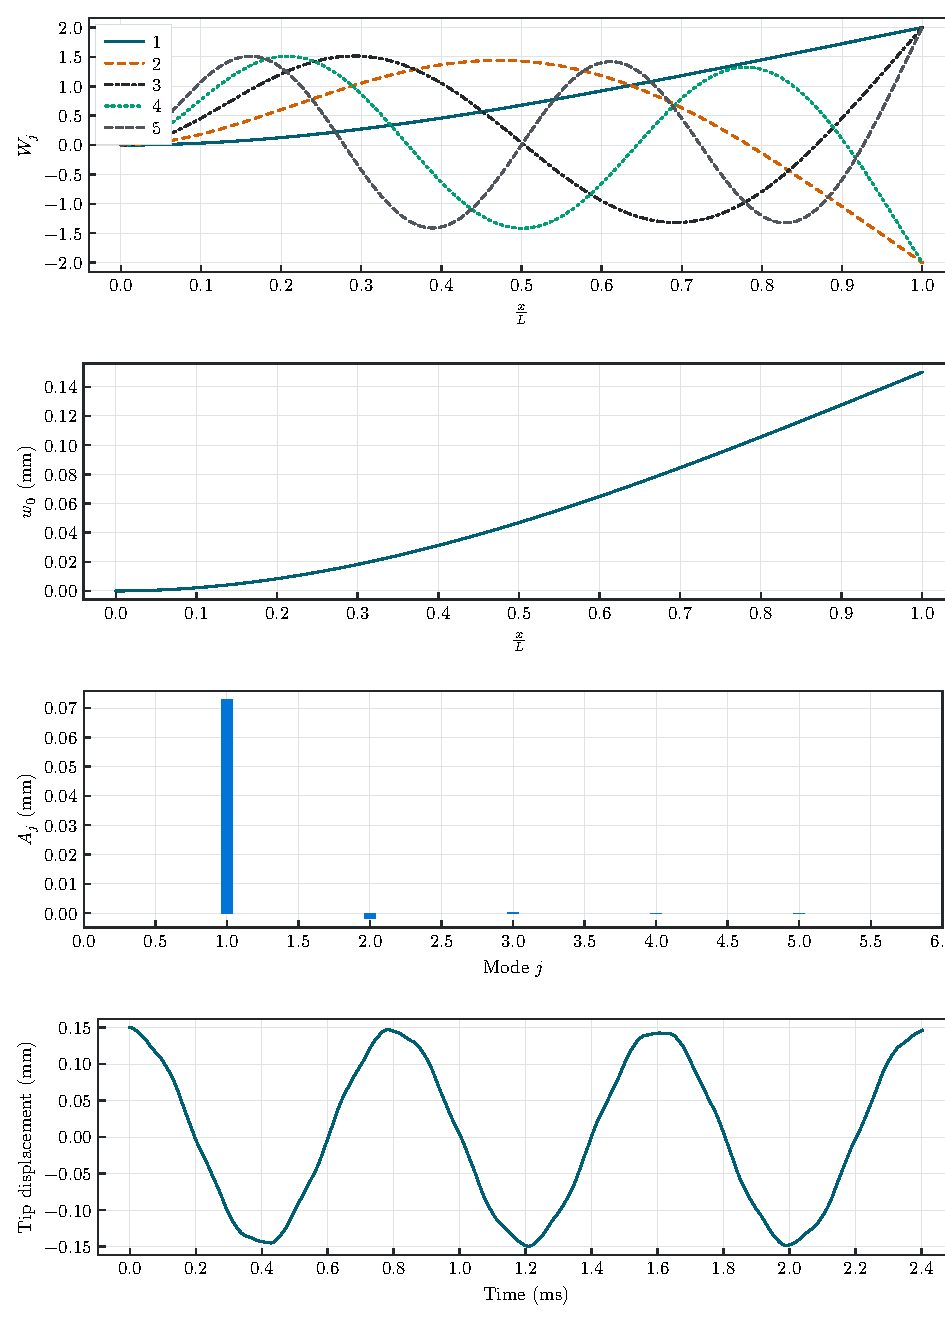
\includegraphics[width=0.82\linewidth]{figures/generated/solutions/B5.pdf}
\caption{B.5. Modes, initial shape, modal coefficients, and tip response over three fundamental periods.}
\end{figure}

\textbf{B.5.9. Interpretation.} The first modal coefficient dominates, so the tip response is close to the fundamental oscillation. The higher modes add small, faster variations. The five-mode initial tip displacement is $0.14995\ \mathrm{mm}$, close to the imposed $0.150\ \mathrm{mm}$.

\lstinputlisting[style=hwmatlab,caption={B.5 MATLAB calculations.}]{matlab/B5.m}
